%        File: 2017-bw-report.tex
%     Created: Fri Aug 11 11:00 AM 2017 C
% Last Change: Fri Aug 11 11:00 AM 2017 C
%
\documentclass[letterpaper]{article}
\usepackage[top=1.0in,bottom=1.0in,left=1.0in,right=1.0in]{geometry}
\usepackage{verbatim}
\usepackage{amssymb}
\usepackage{graphicx}
\usepackage{longtable}
\usepackage{amsfonts}
\usepackage{amsmath}
\usepackage{placeins}
\usepackage[hidelinks]{hyperref}

\author{Kathryn Huff
\\ \href{mailto:kdhuff@illinois.edu}{\texttt{khuff@illinois.edu}}
}

\date{}
\title{Blue Waters Professor Report:\\
Advanced Reactors and Fuel Cycles}
\begin{document}
\maketitle

\section{Project Information}

\paragraph{Project title:} Advanced Reactors and Fuel Cycles

\paragraph{Principal Investigator:} Kathryn Huff, Blue Waters Assistant Professor, Department of Nuclear, Plasma and Radiological Engineering, NCSA Affiliate Faculty, University of Illinois at Urbana-Champaign (kdhuff@illinois.edu)
\paragraph{Co-PIs and Collaborators:} Postdoctoral Scholar Alexander Lindsay was a key part of my research group in 2016-2017:
Alexander Lindsay, Postdoctoral Scholar, Nuclear Plasma and Radiological Engineering, University of Illinois at Urbana-Champaign

\section{Executive Summary}
%Executive summary (150 words)
The Advanced Reactors and Fuel Cycles Group (ARFC) conducts modeling and
simulation in the context of nuclear reactors and fuel cycles toward improved
safety and sustainability of nuclear power. In the context of high performance
computing, this work requires the coupling of multiple physics at multiple
scales to model and simulate the design, safety, and performance of advanced
nuclear reactors. In particular, thermal-hydraulic phenomena, neutron
transport, and fuel performance couple tightly in nuclear reactors. Detailed
spatially and temporally resolved neutron flux and temperature distributions in
particular can improve designs, help characterize performance, inform reactor
safety margins, and enable validation of numerical modeling techniques for
those unique physics. In the work presented here, ARFC has demonstrated the
capability to simulate coupled, transient neutronics and thermal hydraulics in
an advanced, molten-salt-fueled nuclear reactor. 

\section{Description of research activities and results}

ARFC Blue Waters activity began in November 2016 when access to the ARFC 
allocation was initiated for PI Huff.  In the ten months since the start of 
this allocation, Blue Waters has enabled ARFC to develop and test a first of 
its kind finite element model of the transient neutronics and thermal 
hydraulics in a liquid-fueled molten salt reactor design 
\cite{lindsay_moltres_2017}. 

\subsection{Key Challenges:}
The current state of the art in advanced nuclear reactor simulation (e.g. the
CASL DOE innovation hub) is focused on more traditional light water reactors.
This work extends that state of the art by enabling similarly high fidelity
modeling and simulation of more advanced reactor designs which have the
potential to improve the already unparalleled safety and sustainability of
nuclear power. High fidelity simulation of performance in these designs
requires development of models and tools for representing unique materials,
geometries, and physical phenomena.  The current work includes extension of the
MOOSE framework to appropriately model coupled thermal-hydraulics and
neutronics of molten salt flow in a high temperature liquid-fueled reactor
design. Future work will include similarly challenging materials and geometries
such as those in sodium cooled, gas cooled, and very high temperature reactor
designs which promise advanced safety or sustainability.

\subsection{Why it Matters:} 

%description of the potential impact of solving this research problem, and, if 
%appropriate, the educational outcomes. For exploratory allocations, indicate 
%whether the results will be used to substantiate a future proposal.

Nuclear power is an emissions free, safe source of electricity with
unparalleled energy density, baseload capacity, and land-use effiency. 
As we together face energy poverty, climate change, and simultaneous increase
in worldwide energy use, the world's energy future increasingly depends on
improved safety and sustainability of nuclear reactor designs and fuel cycle
strategies. Advanced reactor and fuel cycle systems are sufficiently complex
that sophisticated scientific software so high-performance computing resources
are essential to understanding and improving them.

In particular, insights coupling feedback between the reactor scale and the
fuel cycle scale are essential to the deployment and scalability of these
innovations in the real world. The work conducted in this allocation seeks
exactly those insights and builds a research program that trains future
reactor and fuel cycle designers in best practices for large scale engineering 
modeling and simulation. Additionally, development and demonstration
of high fidelity software for multi-physics in advanced reactor types builds a
foundation for future funding through the Department of Energy Office of
Nuclear Energy. 


\subsection{Why Blue Waters:} To assess nuclear reactor performance under a
variety of conditions and dynamic transients, the ARFC group must conduct
myriad 2-dimensional and 3-dimensional finite element simulations using the
MOOSE framework and our in-house developed modules. This class of simulations commonly
occupy tens of thousands of CPU cores at a time and vary in completion time.
The MOOSE framework is shown to scale very well up to 10,000 cores. The ARFC
group has demonstrated appropriate scaling for MSR simulation above 20,000 CPU
cores (600 Blue Waters nodes). Transient and multi-scale simulations, which
require greater capability per simulation, are on the horizon for our work.
These may occupy up to 100,000 CPU cores at a time. Only a few of those larger
simulations will be necessary to enable better understanding of the dynamics in
these reactor systems.

\subsection{Accomplishments:} 
Moltres \cite{lindsay_moltres_2016} is
a physics application for multiphysics modeling of fluid-fuelled molten salt
reactors (MSRs). It couples equations for neutron diffusion, thermal
hydraulics, and delayed neutron precursor transport. Neutron diffusion and
precursor transport equations are set up using an action system that allows the
user to use an arbitrary number of neutron energy and precursor groups
respectively with minimal input changes. Moltres sits atop the Multi-physics
Object-Oriented Simulation Environment \cite{gaston_moose_2010} which gives it the
capability to run seamlessly in massively parallel environments. To date,
Moltres has been used to simulate MSRs in 2D-axisymmetric and 3D geometric
configurations. As these simulations increase in fidelity, their results will
be able to inform the safety and sustainability case for deployment of advanced
commercial nuclear reactors.

Moltres solves arbitrary-group neutron diffusion, temperature, and precursor
governing equations in anywhere from one to three dimensions and can be
deployed on an arbitrary number of processing units. The model problem
presented here has a 2D-axisymmetric geometry with heterogeneous group
constants for fuel and moderator regions. Fuel volume fraction and fuel salt
composition are based on the Molten Salt Reactor Experiment design. Figure 
\ref{fig:flux} demonstrates that neutron
fluxes show expected cosinusoidal shapes in radial and axial directions with
visible striations between fuel and moderator regions. The fast group flux is
enhanced in fuel regions while the thermal group flux in enhanced in moderator
regions. 

\begin{figure}[htb]
        \begin{center}
                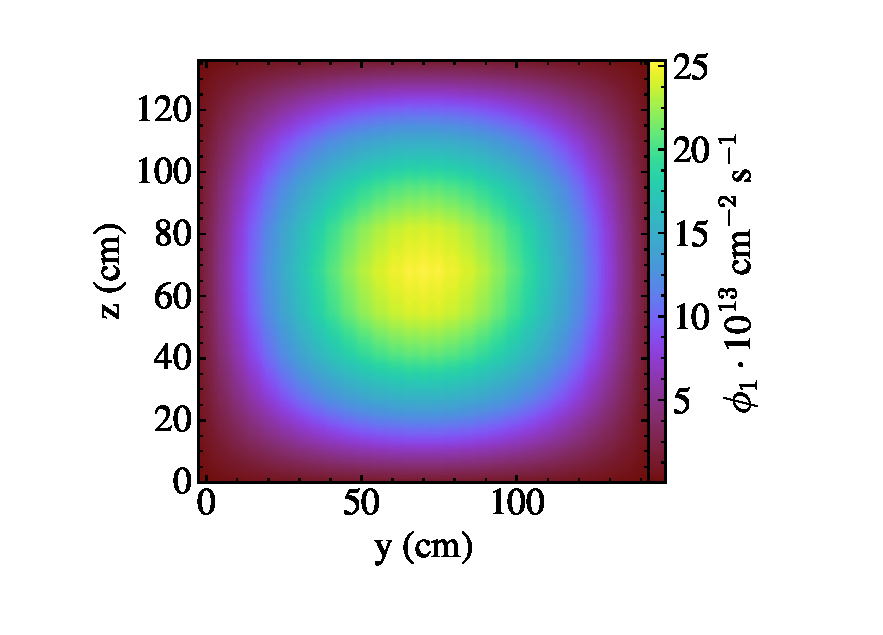
\includegraphics[width=0.5\textwidth]{flux.eps}
        \end{center}
        \caption{This image shows the neutron flux in a 2-D cylindrical axisymmetric model of an MSR. This flux has the anticipated magnitude and canonical cosine shape (r = 0 is center of core) and is undergoing validation against experimental results from the Molten Salt Reactor Experiment.}
        \label{fig:flux}
\end{figure}

In Figure \ref{fig:temp}, it can be seen that the temperature profile increases monotonically in
the direction of salt flow. This is due to advection. 

\begin{figure}[htb]
        \begin{center}
                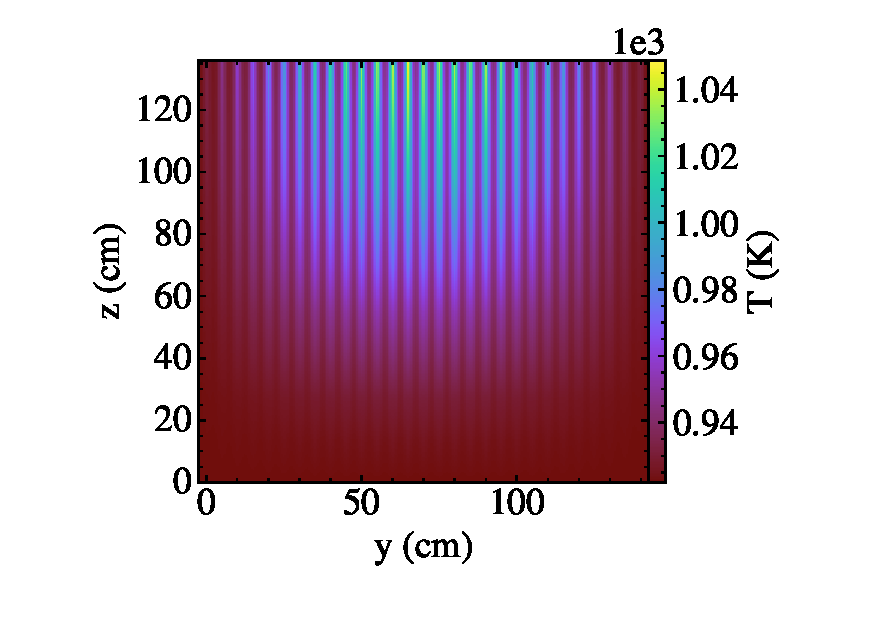
\includegraphics[width=0.5\textwidth]{temp.eps}
        \end{center}
        \caption{This image shows the temperature in a 2-D cylindrical axisymmetric model of an MSR. The reactor core temperature peaks near the reactor outlet in this 2-D axisymmetric model because of fuel advection (r = 0 is center of core).} 
        \label{fig:temp}
\end{figure}

The role of advection is also seen in precursor
concentrations. Long lived precursors exhibit maximum concentrations at the
core outlet, as seen in Figure \ref{fig:pre1}


\begin{figure}[htb]
        \begin{center}
                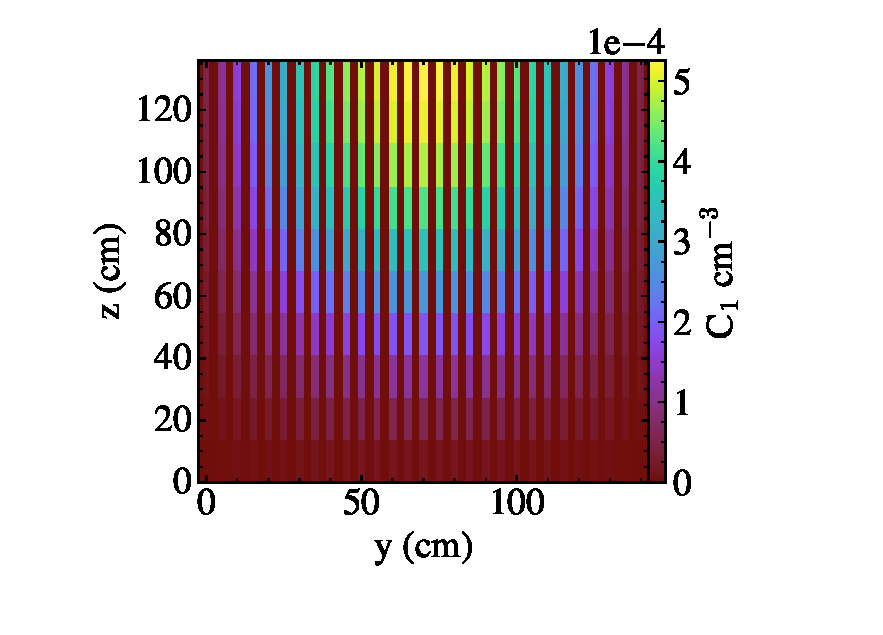
\includegraphics[width=0.5\textwidth]{pre1.eps}
        \end{center}
        \caption{This image shows the concentration of some particularly 
        important fission-product nuclides called delayed neutron precursors.  
        The concentration of the group of longest lived precursors ($\lambda = 
        1.24\times{10}^{-2}{s}^{-1}$) peaks near the reactor outlet in this 2-D 
        axisymmetric model (r = 0 is center of core).} 
        \label{fig:pre1}
\end{figure}

As the decay constant increases across precursor groups the maximum
concentrations moves towards the reactor center where the precursor production
rate is maximum. Future Moltres work includes generating a high-fidelity 3D
model as well as investigating various transient accident scenarios.
\FloatBarrier

\section{List of publications associated with this work}

%List any publications and products (including papers in-preparation and 
%submitted, posters, and curricular materials that can be made available to the 
%community). Indicate the current state (work in progress/submitted/published). 
%If available, please include the DOI for published works.

%Highlight any keynote or other presentations that featured your work on Blue Waters.


\subsection{Highlighted Keynotes} I gave two keynote talks 
this year. One was to PyCon 2017, with an audience of over 3000 people. The 
second was at SciPy 2017, with an audience of 700 people. Each keynote 
mentioned my affiliation with NCSA, my position as a Blue Waters Professor, and 
the work being conducted on Blue Waters in my group. 

\begin{itemize}
\item Kathryn Huff, ``Academic Open Source'' Scientific Python Conference 
(SciPy2017), Austin, TX. July 12, 2017.  
Presentation: \url{http://katyhuff.github.io/2017-07-12-scipy}. Video: 
\url{https://www.youtube.com/watch?v=Nqzvnqg4OJ8}.
\item Kathryn Huff, ``Do it for Science'' Python Conference (PyCon2017),
Portland, OR, May 20, 2017. Presentation: \url{http://katyhuff.github.io/2017-05-20-pycon}.
Video: \url{https://www.youtube.com/watch?v=kaGS4YXwciQ}.
\end{itemize}

\subsection{Highlighted Presentations} The work conducted on Blue Waters using 
Moltres appeared in detail within three presentations during the course of the 
allocation. 

\begin{itemize}
\item Alexander Lindsay and Kathryn Huff, ``Moltres: a MOOSE Application for
Simulation of MSRs.'' Workshop on Multi-physics Modeling and Simulation of
Molten Salt Reactors, Berkeley, CA.June 15, 2017. Presentation:
\url{arfc.npre.illinois.edu/img/pres/2017-06-15-msr-pres.pdf}.
\item Kathryn Huff, ``Modeling and Simulation of Advanced Reactors and Fuel
Cycles,'' Invited Seminar, UC Davis Mechanical and Aerospace Engineering
Seminar, Davis, CA. April 20, 2017. Presentation:
\url{http://katyhuff.github.io/2017-04-20-davis}. Video:
\url{https://www.youtube.com/watch?v=YqTxZC1i-B0#t=6m28s}
\item Kathryn Huff, ``Advanced Nuclear Reactors and Fuel Cycles: Simulation of 
        Multiple Physics at Disparate Scales'' Computational Science and 
                Engineering Seminar Series, 1030 National Center for 
                Supercomputing Applications, Urbana, IL Presentation: 
                \url{http://katyhuff.github.io/2017-02-02-cse}.  Video: 
                \url{https://www.youtube.com/watch?v=fWlUW_CFo3M}.
\end{itemize}
\section{Plan for next year}

The development of this software  began in September 2016 and has now been
demonstrated on hundreds of nodes on blue waters. We will scale it up to much
larger problems very soon.

\begin{figure}[htbp!]
\begin{center}
        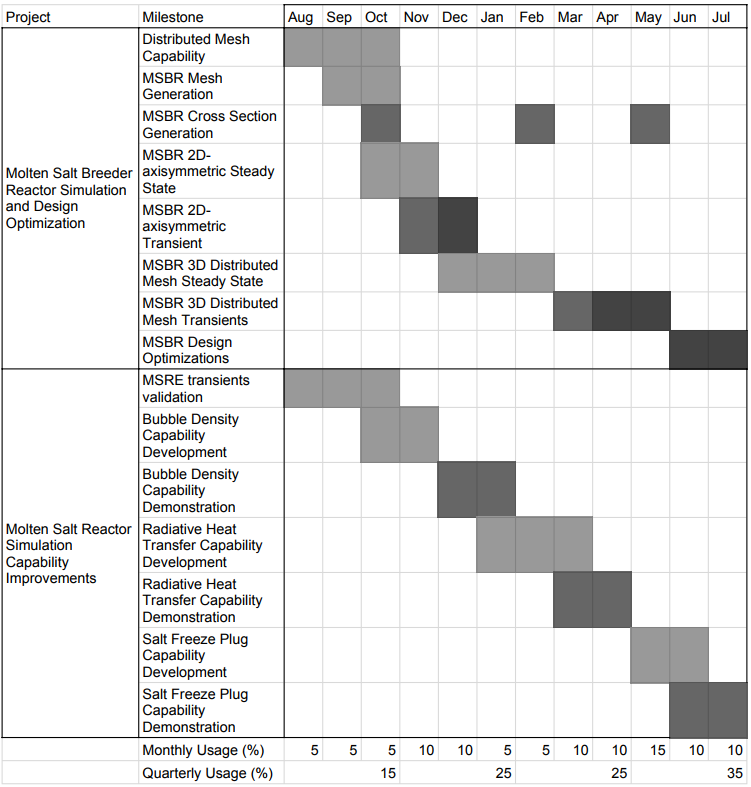
\includegraphics[width=\textwidth]{proj.png}
\end{center}
\caption{Planned project schedule for molten salt reactor related activities in 2017-2018.}
\label{fig:proj}
\end{figure}

The following 

\begin{itemize}
        \item \textbf{Larger Scale Problems} The software we developed in house (moltres) is now capable of 3D 
        simulation. Its performance is currently memory constrained. 
               Distributed Mesh memory handling will be implemented in the near 
                term in order to overcome this barrier. 
        \item \textbf{Monte-Carlo Cross-Section Generation} The ARFC group intends to begin working with monte-carlo software for 
        cross section generation. Ideally, we would like to run Serpent 2 or 
                OpenMC. The Serpent 2 software is fully parallelizable, very 
                memory intensive, and will produce very high fidelity results. 
                If we are able to use it on Blue Waters, the quality of our 
                results will improve enormously, as will the computational 
                intensity of our work.
\item \textbf{Quadrupling Group Size} The number of graduate students in the Advanced Reactors and Fuel Cycles
        \item \textbf{Expansion into Agent Based Modeling} The scope of the work within ARFC will be expanded to include some capacity
computing work. While this is not the bulk of ARFC work, we have a project in
statistical optimization methods for agent based modeling which could benefit
from a few hundreds or thousands of independent single-node runs. 
group will quadruple this year, from 2 to 8. 
\end{itemize}

\paragraph{System nodes needed per run:} 20 - 2,000. Many simulations will be 
run on 100-200 nodes, while a few much larger simulations will be run on 2,000 
nodes. While it is possible, it is unlikely that we will run larger runs 
this year.
\paragraph{Anticipated memory usage:}
\paragraph{Expected numerical operations}
\paragraph{Expected local and remote memory accesses}
\paragraph{Total Node Hours}
\paragraph{Anticipated input and output requirements}
\paragraph{Anticipated data transfer}

%Describe the Blue Waters resources required for next year. This description 
%should include the number of system nodes needed for your runs, the 
%anticipated actual memory usage, the expected numbers of each major class of 
%arithmetic and logical operation, the expected numbers of local and remote 
%memory accesses, the total number of node-hours required, the anticipated 
%input and output requirements, the amount of data that you anticipate 
%transferring to or from the Blue Waters enclave, the amount and type of 
%storage required and any other system resource needs that you anticipate

%For assistance in computing node hours for Blue Waters see: 
%https://bluewaters.ncsa.illinois.edu/node\_core\_comparison

%For a description of the default storage quotas see: 
%https://bluewaters.ncsa.illinois.edu/storage. If your project will require 
%storage limits that exceed the standard quotas, provide a justification in 
%support of your request.

\subsection{Usage Schedule:} See Figure \ref{fig:proj}.
%Provide an estimated Blue Waters usage schedule. The estimate should be per 
%quarter and may be represented as a percent of the requested allocation (e.g. 
%Q1: 10\%, Q2: 20\%, Q3: 50\%, Q4: 20\%).

 

%The report should be submitted as a PDF file. There are no specific formatting 
%instructions. It is recommended to include visualizations, charts and other 
%images in the document to help illustrate the results. 

%If you have questions, please contact Jay Roloff at cesc@ncsa.illinois.edu or 
%the Blue Waters support staff at help+bw@ncsa.illinois.edu.

\pagebreak
\bibliographystyle{ieeetr}
\bibliography{2017-bw-report}


\end{document}


